\documentclass[lettersize,journal]{IEEEtran}
% \documentclass[draftcls,onecolumn]{IEEEtran}
\usepackage{amsmath,amsfonts}
\usepackage{algorithmic}
\usepackage{algorithm}
\usepackage{array}
\usepackage[caption=false,font=normalsize,labelfont=sf,textfont=sf]{subfig}
\usepackage{textcomp}
\usepackage{stfloats}
\usepackage{url}
\usepackage{verbatim}
\usepackage{graphicx}
\usepackage{cite}
\usepackage{color}
\usepackage{hyperref}
%\usepackage{subcaption}
% \usepackage{subfigure}
\usepackage{caption}
\usepackage{booktabs}
\usepackage{multirow,makecell}
\usepackage{bm}
\usepackage{amssymb}
\usepackage{amsthm}
\usepackage{adjustbox}
\usepackage{tabularx}
\usepackage{float}
\usepackage[scr=rsfs]{mathalpha}
\usepackage{threeparttable} 
\usepackage{lineno}
\hyphenation{op-tical net-works semi-conduc-tor IEEE-Xplore}
% updated with editorial comments 8/9/2021

\begin{document}
% \pagewiselinenumbers
% \switchlinenumbers
\title{A Robust Attention Based Land Cover Classification Scheme for Corrupted Remote Sensing Images
}

\author{Weipeng Shi, Wenhu Qin$^{*}$, Zhonghua Yun, Tao Zhao, Chao Wu, Allshine Chen
    % <-this % stops a space
    \thanks{This work was supported by Key R\&D Program of Jiangsu Province under Grant BE2019311, Jiangsu modern agricultural industry key technology innovation project under Grant CX(20)2013 and
        National key research and development program under Grant
        2020YFB160070301. Weipeng Shi\emph{(bowenroom1@gmail.com)}, Wenhu Qin$^{*}$\emph{(corresponding author, qinwenhu@seu.edu.cn)}, Zhonghua Yun,  Chao Wu are with School of Instrument Science and Engineering, Southeast University, Nanjing, 210096, China. Allshine Chen is with Health Sciences Center, University of Oklahoma, Oklahoma City, 73106, USA. Tao Zhao is with Institute of Intelligent Manufacturing, Nanjing Tech University, Nanjing 210009, China.}% <-this % stops a space
}

% The paper headers
\markboth{IEEE Geoscience and Remote Sensing Letters}%
{Weipeng Shi \MakeLowercase{\textit{et al.}}:A Robust Attention Based Land Cover Classification Scheme for Corrupted Remote Sensing Images}

% \IEEEpubid{0000--0000/00\$00.00~\copyright~2021 IEEE}
% Remember, if you use this you must call \IEEEpubidadjcol in the second
% column for its text to clear the IEEEpubid mark.

\maketitle

\begin{abstract}
    There is a significant effect of deep learning on the accuracy of land cover classification. Nonetheless, there is always a notable reduction of classification robustness in foggy conditions, which is commonly overlooked. Several challenging factors, like low image quality and occlusion, contribute to this. Instead of focusing solely on classification accuracy, we also explore the influence of attention mechanisms and multimodal fusion on classification robustness. ConvNeXt is adopted as the backbone. Furthermore, we propose Contextual Representation Enhancement Module (CREM) and Cross-Modal Fusion Module (CMFM) based on nonlocal operation. CREM possesses a large perceptive field to fuse local and global features, reducing side effects of the redundant noise. CMFM explores the relationship between multimodal inputs for information recalibration. Extensive ablation and comparison experiments were conducted on the corrupted ISPRS Potsdam and Vaihingen benchmark datasets to validate the proposed method. Compared to the reference model, our framework exhibits excellent accuracy and robustness in the task of land cover classification. Code will be available at \href{https://github.com/bowenroom/Robust-land-cover-classification}{https://github.com/bowenroom/Robust-land-cover-classification}.
\end{abstract}

\begin{IEEEkeywords}
    Semantic segmentation, Attention mechanism, Robust deep learning, Remote sensing, Data fusion
\end{IEEEkeywords}

\section{INTRODUCTION}
Accurate and robust land cover classification (LCC, a.k.a. semantic segmentation) of remote sensing images (RSIs) is a prerequisite for a series of tasks, such as earth observation\cite{Schmitt2019SEN12MSA}, crop growth monitoring\cite{Mandal2020DualPR}, soil-permittivity estimation \cite{Hnsch2021SoilPermittivityEU} and so on. Models with high robustness perform well on fog corrupted RSIs with less degradation compared to the clean. In general, LCC models, which apply deep learning with positive results, can be categorized into four types: FCNs\cite{shelhamerFullyConvolutionalNetworks2017}, UNets\cite{ronnebergerUNetConvolutionalNetworks2015}, HRNets\cite{wangDeepHighResolutionRepresentation2020}, and ViTs\cite{liuSwinTransformerHierarchical2021}. Despite the availability on clean data, they are not always reliable when corruptions exist.

 Figure.\ref{challenges} illustrates some frequently encountered challenges in foggy conditions. It is evident from Figure.\ref{challenges}(a) that there is a distinction in shapes of the cars. The fog interferes with visual representations of heterogeneous objects, resulting in a high degree of homogeneity in Figure.\ref{challenges}(b) (d) (e). In Figure.\ref{challenges}(c), a large proportion of the car is heavily obscured by trees and fog. It is tough to distinguish homogeneous cars in Figure.\ref{challenges}(f) as a result of shadows and occlusion.

\begin{figure}[!htbp]
    \centering
    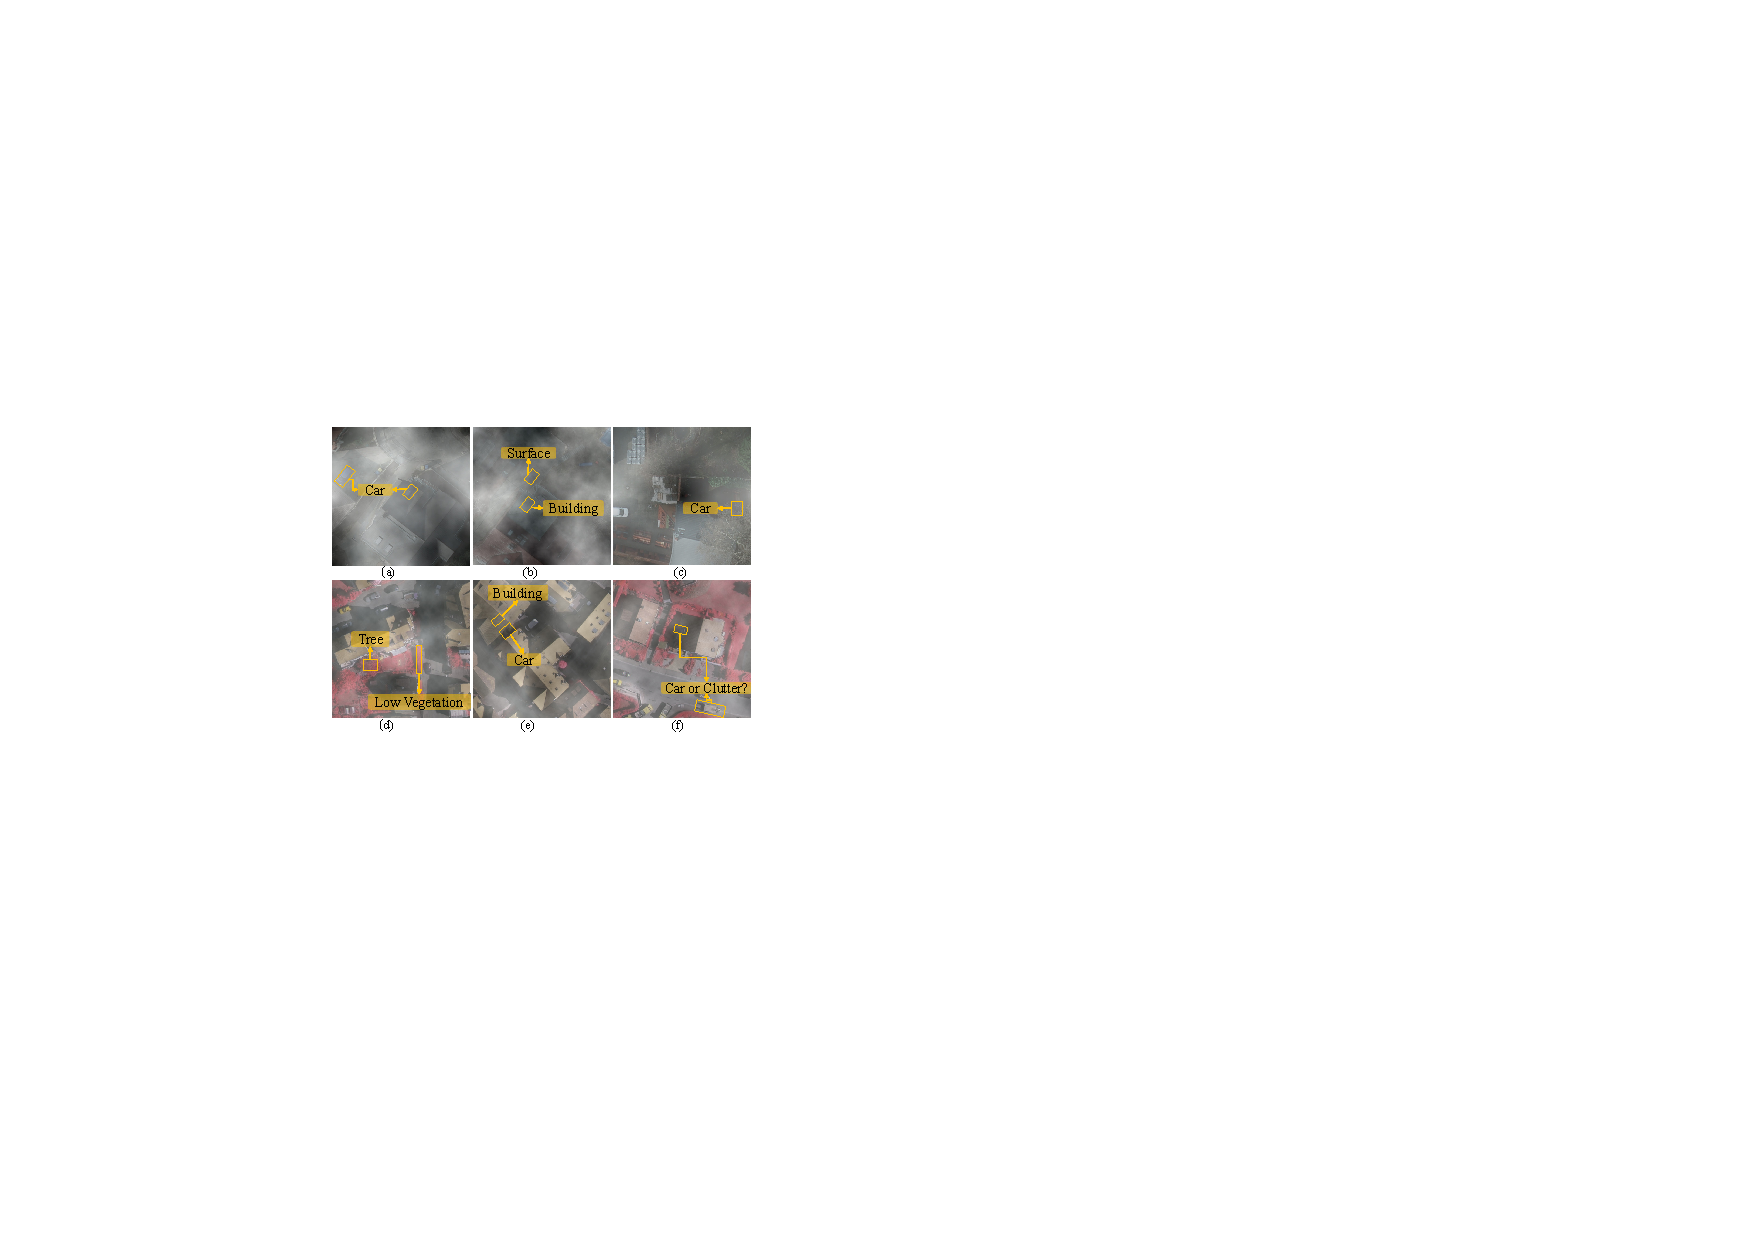
\includegraphics[width=3.5in]{challenges.pdf}
    \caption{Some challenging characteristcs of fog corrupted RSIs, such as diverse scales and shapes, heterogeneous homogeneity, occlusion as well as homogeneous heterogeneity.
    }
    \label{challenges}
    \vspace{-0.2cm}
\end{figure}

\begin{figure*}[!htbp]
    \centering
    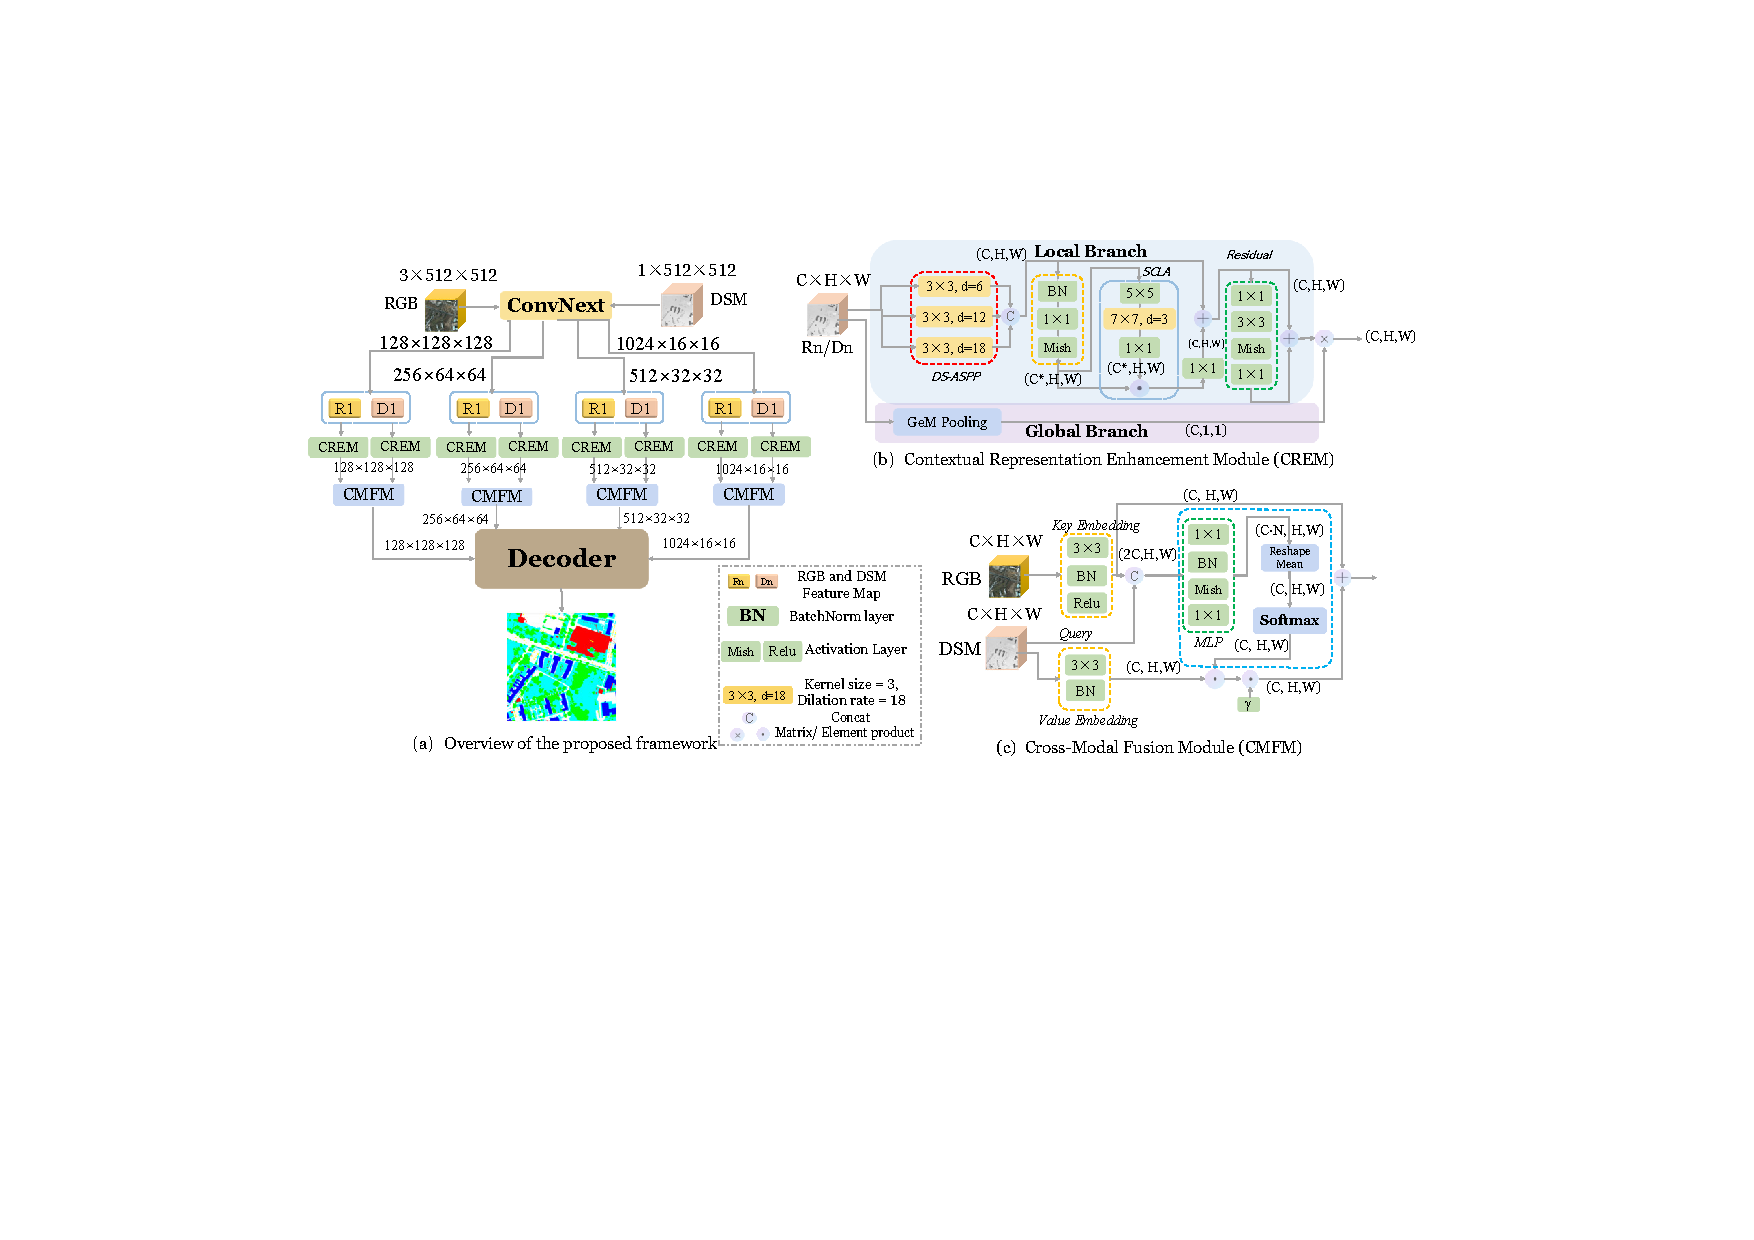
\includegraphics[width=\textwidth]{overall.pdf}
    \caption{Architecture of our model. It is composed of an encoder (ConvNeXt), CREM, CMFM and a decoder (UPerNet).}
    \label{backbone}
    \vspace{-0.2cm}
\end{figure*}

To cope with the challenges encountered in fog, it is imperative to explore how to conduct LCC robustly. In view of the outstanding performance while handling images with poor quality, we adopt ConvNeXt \cite{liuConvNet2020s2022} as the backbone. Meanwhile, we propose and incorporate additional two modules, CREM and CMFM, to improve the robustness. CREM consists of local and global branches. CREM is featured by a large receptive field which captures and integrates global as well as local features to reduce the redundant noise. Based on the non-local operation, we propose CMFM to recalibrate and explore  the complementary interaction between multimodal inputs. In other words, our contributions can be summarized as the following:

\begin{itemize}
    \item  For land cover classification under fog, we develop an end-to-end model to improve the performance without significant degradation comparing to the clean condition.
    \item We propose CREM for feature extraction and CMFM for multimodal fusion based on the backbone ConvNeXt.
    \item A fog corrupted test set is generated for the robustness evaluation of each framework. 
\end{itemize}

\section{METHODOLOGY}
\subsection{Backbone and Decoder}
According to the framework overview in Figure.\ref{backbone}, both modalities are firstly assembled into ConvNeXt for encoding, which generates feature maps with four various resolutions. Low-level features are more exhaustive but contain redundant noise, whereas high-level features are enriched in semantic information but do not depict edges precisely. CREM is proposed to fuse local and global features, while CMFM is conducive to the extractions of complementary representations  from multimodal inputs. According to the comprehensive comparison in \cite{tangRobustARTBenchmarkingRobustness2021}, ResNeXt is capable of handling distorted images properly. In view of inherent inductive bias and translational invariance of CNNs, ConvNeXt, which follows the ResNeXt design scheme of using group convolution to extend model width, is more robust than ViT. Furthermore, equipment of the large kernel convolution provides a large and global receptive field. Therefore, we deploy ConvNeXt as the backbone, which allows the network to effectively cope with low-quality RSIs. UPerNet is selected as the decoder, which implements a top-down lightweight structure accompanied by a feature pyramid network and a pyramid pooling module to exploit hierarchical levels of representations. In the context of complex remote sensing scenarios, the combination of parsed visual attributes improves classification robustness.


\subsection{Context Representation Enhancement Module}
If corrupted multimodal inputs (denoted as \bm{$X$}, $X\in R^{C\times H \times W}$) collected under fog are fed directly to the fusion module, the network will be subject to an increased level of redundancy and noise. To reduce interference of the noise on robustness, we propose CREM, illustrated in Figure.\ref{backbone}, to boost the capability of obtaining useful information. It is composed of local and global branches, which strengthen the complementarity and compatibility between multiple modalities. The acquired global representation is generally more tolerant of variations in illumination and viewing angles in RSIs, while the local representation is more sensitive to edge details, geometry and texture. Calibration fusion filters the noise information. 

The local branch consists of a Depthwise Separable Astrous Spatial Pyramid Pooling (DS-ASPP), a Spatial and Channel Large kernel Attention (SCLA) and a residual module. DS-ASPP can efficiently cope with the scale diversity of instances in RSIs with a marginal cost. Depthwise Separable convolution \cite{howardMobileNetsEfficientConvolutional2017} is comprised of depthwise and pointwise convolutions, where the depthwise performs a separate spatial convolution for each channel and the pointwise combines the generated outputs. After concatenating output from DS-ASPP (denoted as \bm{$X_{aspp}$}, $X_{aspp}\in R^{C\times H \times W}$), the embeded result (\bm{$X_{aspp}^{*}$}, $ X_{aspp}^{*}\in R^{C\times H \times W}$) is acquired by a 1×1 convolution (\bm{$K_{1}^{1\times 1}$}). Self attention mechanism ignores the adaptive characteristics of each channel. We get the attention map (\bm{$X_{scla}$}, $ X_{scla}\in R^{C^{*}\times H \times W}$) after SCLA, which consists of three types of convolution(\bm{$K^{1\times 1}$}, \bm{$K^{DW\_D}$}, \bm{$K^{DW}$ }denote 1×1 convolution, depth-wise dilation convolution, depth-wise convolution respectively). A 1×1 convolution is applied for channel alignment. The fused result (\bm{$\hat{X}_{scla} $}, $ \hat{X}_{scla} \in R^{C\times H \times W}$) can model the importance of each channel and location in feature maps, thus capturing the long-range dependencies in RSIs well. Summed with the original input, we use a residual module to reduce the information redundancy. \bm{$Y_{glocal}$} $(Y\in R^{C\times 1 \times 1})$ is the feature map after generalized-mean pooling layer (GeM Pooling\cite{yangDOLGSingleStageImage2021}), which can generate an image descriptor about spatial distribution of distinction influence. $p_{n}$ is the pooling parameter, controlling amount of the response correspondence. $\otimes$ denotes the element-wise product. Therefore, we could explore the complementary context through matrix product fusion of two branches. Formula details are displayed as the following:

\begin{equation}
    \mathbf{X}_{aspp}^{*}=\mathbf{K_{1}}^{1\times 1} \cdot \mathbf{X}_{aspp}
    \label{eqASPP}
\end{equation}

\begin{equation}
    X_{scla} =  \mathbf{K_{2}^{1\times 1}} \cdot \mathbf{K^{DW\_D}} \cdot \mathbf{K^{DW}} \cdot \mathbf{X}_{aspp}^{*}
    \label{eqSCLA}
\end{equation}

\begin{equation}
    \hat{X}_{scla} =  \mathbf{K_{3}^{1\times 1}} \cdot (\mathbf{X}_{aspp}^{*} \otimes X_{scla})+ \mathbf{X}_{aspp}
    \label{eqFuse}
\end{equation}
\begin{equation}
    \mathbf{Y_{local}} = {\mathbf{F}}(\hat{X}_{scla}) +\hat{X}_{scla}
    \label{eqOutput}
\end{equation}
    \begin{equation}
    \resizebox{0.91\hsize}{!}{ $  \mathbf{Y_{global}}=\left[\mathrm{y}_{1}^{(g)} \ldots \mathrm{y}_{n}^{(g)} \ldots \mathrm{y}_{C}^{(g)}\right]^{\top},\mathrm{y}_{n}^{(g)}=\left(\frac{1}{\left|\mathcal{X}_{n}\right|} \sum_{x \in \mathcal{X}_{n}} x^{p_{n}}\right)^{\frac{1}{p_{n}}} $  }
        \label{eqGEM}
    \end{equation}

\subsection{Cross-Modal Fusion Module}
Conventional early-fusion algorithm fuse multimodal data ineffectively, since it can not acquire interactive characteristics and relationship between modalities adequately. Self-attention scheme efficiently activates the feature map which is associated with various spatial locations of inputs. Figure.\ref{backbone} illustrates CMFM. Rather than purely relying on self-attention, we combine contextual information from RGB input (\bm{$X_{RGB}$}, $X_{RGB}\in R^{C\times H \times W}$) with sparse, high-quality height information from DSM (\bm{$X_{DSM}$}, $X_{DSM}\in R^{C\times H \times W}$).  Consequently,  the relationship between adjacent context can be effectively exploited, resulting in an aggregated output.

The key embedding is based on $3\times 3$ depth-wise convolution $W_k^{D}$, which contextualizes the key representation over spatial locations. We then acquire the attention matrix  \bm{$Y_{attn}$} by passing concatenated feature maps through MLP. The embeded key feature map  $W_k^{D} X_{RGB}$ acts as the static context, which guides the key learning points. $\gamma$ is the learnable scalar initiallizing from 0, which controls the weight of dynamic contextual representation. Utilizing element-sum, we explore complementary interactions of multimodal inputs. This process is formulated as:
    \begin{equation}
        \mathbf{Y_{attn}} = W_{mlp} \cdot [Concat(W_k^{D} X_{RGB}, X_{DSM})]
        \label{eqAttn}
    \end{equation}

    \begin{equation}
        \resizebox{0.9\hsize}{!}{$
        \mathbf{Y_{output}} =W_k^{D} X_{RGB} + \gamma \cdot [Softmax(Y_{attn})\cdot W_{q}X_{DSM} ] $}
        \label{eqCMFM}
    \end{equation}

\section{EXPERIMENTS AND ANALYSIS}
\subsection{Dataset}\label{sec:dataset}
ISPRS\footnote{Potsdam and Vaihingen datasets can be acquired from \emph{https://www.isprs.org/education/benchmarks/UrbanSemLab/2d-sem-label-potsdam.aspx} and \emph{https://www.isprs.org/education/benchmarks/UrbanSemLab/2d-sem-label-vaihingen.aspx} (\emph{{Accessed in June, 2022})}} offers Potsdam and Vaihingen LCC datasets for the experiment. Potsdam has a resolution and ground sampling distance of $6000\times 6000$ pixels and 5cm respectively.
Corresponding parameters for Vaihingen are $2500\times 2500$ pixels and 9cm. Image in Potsdam indexed \textbf{4\_12} was removed as a result of the error existing in the annotation. In accordance with the ratio of 0.8, 0.1, and 0.1, each dataset is divided into a training set, a validation set, and a test set.
Building, Car, Vegetation, Tree, Surface as well as Clutter make up the entire dataset. Figure.\ref{imbalance} demonstrates the proportion of different classes in both aerial datasets. In Figure.\ref{imbalance}, it is clear that buildings accompanied by the impervious surface account for more than half of all pixels. The percentage of Car is considerably inferior to the other items. Clutter in Potsdam is 7.4 times greater than in Vaihingen. This phenomenon arises from the complicated attribute of city scenes.

Data augmentation techniques, including random rotation, reflection padding, random adjustment of basic attributes and so on, are applied to reduce overfitting and class imbalance issues. The original image, which is captured in normal conditions, is applied for model training and validation. To evaluate the robustness performance in various circumstances, we create the fog corrupted dataset based on diamond-square algorithm \cite{kamannBenchmarkingRobustnessSemantic2021}. Figure.\ref{fogSeverity} displays several conditions with different degrees of fog corruptions.

\begin{figure}[!htbp]
    \centering
    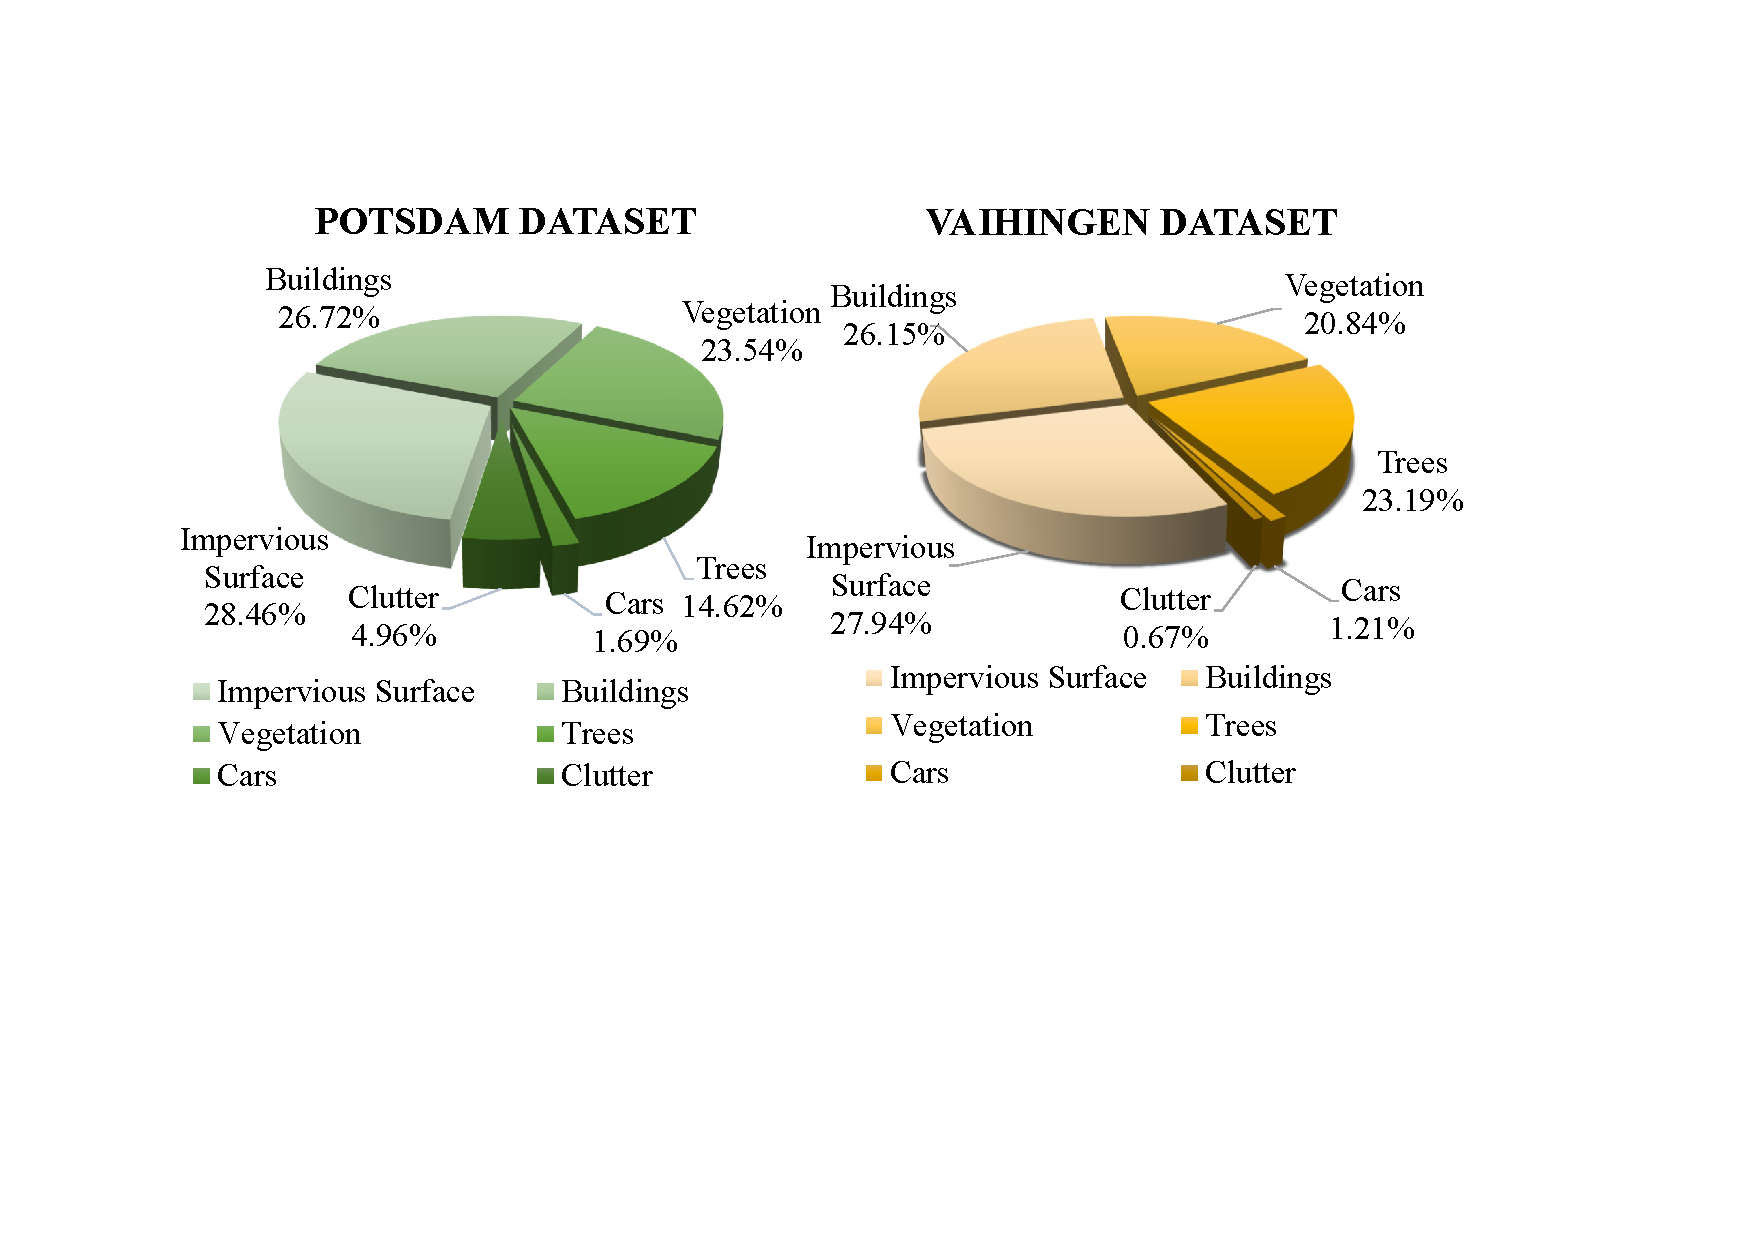
\includegraphics[width=3.5in]{dataset.pdf}
    \caption{Class imbalance exists in both datasets.}
    \label{imbalance}
    \vspace{-0.2cm}
\end{figure}

\begin{figure}[!htbp]
    \centering
    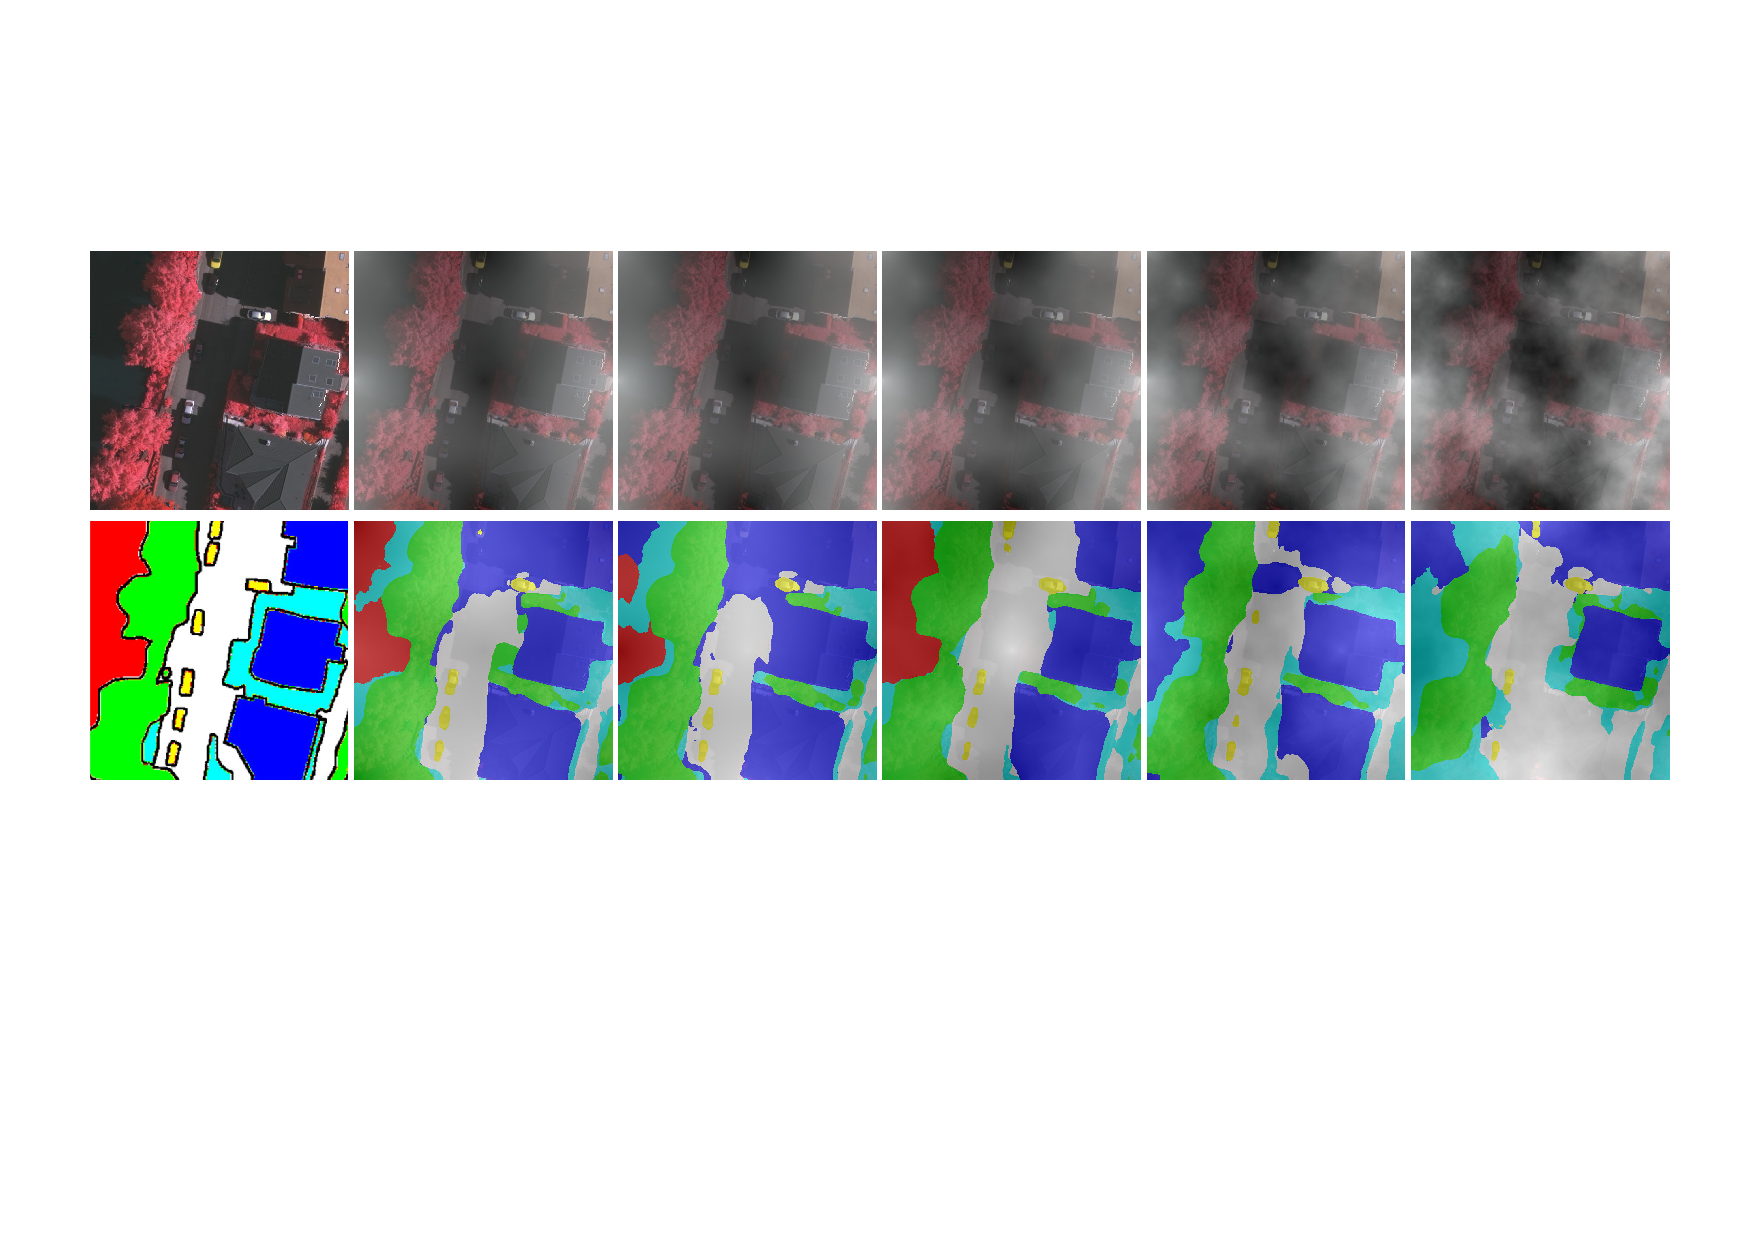
\includegraphics[width=\columnwidth]{fogSeverity}
    \caption{The first column displays a clean Vaihingen image with the ground truth. Fog concentration gradually increases from left to right and the second row corresponds to LCC result.}
    \label{fogSeverity}
    \vspace{-0.5cm}
\end{figure}
\subsection{Metrics}
Metrics utilized to evaluate the performance are F1 score (\textbf{$F1_{score}$}), Overall Accuracy (\textbf{OA}). Corruption Degradation (\textbf{CD}). We define \bm{$CD$}\cite{kamannBenchmarkingRobustnessSemantic2021}  and Degradation \bm{$D$} as the following:
\begin{small}
    \begin{equation}
        D=1- F1_{score}
        \label{Degradation}
    \end{equation}
    \begin{equation}
        CD^{f}=\frac{\widetilde{D^{f}}}{\widetilde{{D}^{r e f}}}\times 100\%
        \label{CD}
    \end{equation}
\end{small}

Specifically speaking,  \emph{$OA$} as well as \emph{$F1_{score}$} are to evaluate LCC accuracy and CD assesses LCC robustness in terms of various fog corruptions. Larger values of \emph{$OA$} and \emph{$F1_{score}$} indicate the better performance in LCC accuracy, whereas larger \emph{CD} value represents a lower robustness with higher LCC performance degradation. \emph{ref} and \emph{f} denote the reference and selected models. \emph{D} represents the absolute robustness degradation where $\widetilde{D^{f}}$ indicates the average degradation over various levels of fog corruption. 

\subsection{Implementation Details}
Training and inference are performed on one RTX 3090. To fit into GPU memory, we slice the high-resolution image into 512x512 pixels. 
We assemble RGB and DSM into one image by means of RGB channels and alpha channel. Mish activation is also adopted in Figure.\ref{backbone} \cite{Misra2020MishAS}. Dilation rates in DS-ASPP are [6,12,18]. $C^{*}$, $N$, $p_{n}$ in Figure.\ref{backbone} and Equation.\eqref{eqGEM} are set as 300, 3, 32 respectively. 
 With blocks of [3, 3, 27, 3] for each stage, ConvNeXt (\textbf{Base}) pretrained on ImageNet is adopted as the backbone and we take UperNet as the decoder. The learning rate is set initially as 1e-4 using a poly learning rate schedule with a power of 1. Weight decay is 5e-2. To reduce the memory consumption, we  train each model in 40k iterations with the mixed precision training strategy. 

 % Table generated by Excel2LaTeX from sheet 'ablation'
\begin{table}[!htbp]
    \centering
    \LARGE
    \caption{Ablation study of CREM on Potsdam dataset}
    \begin{adjustbox}{width=1\columnwidth}
      \begin{tabular}{c|c|c|c|c|cc|c}
      \hline
      \multirow{2}[4]{*}{\textbf{Index}} & \multirow{2}[4]{*}{\textbf{Backbone}} & \multicolumn{3}{c|}{\textbf{CREM}} & \multicolumn{2}{c|}{\textbf{mFscore(\%)↑}} & \multirow{2}[4]{*}{\textbf{CD(\%) ↓}} \\
  \cline{3-7}          &       & \multicolumn{1}{p{5.11em}|}{\textbf{DS-ASPP}} & \textbf{SCLA} & \multicolumn{1}{p{5em}|}{\textbf{GEM-P}} & \textbf{Clean} & \textbf{Fog} &  \\
      \hline
      A     & \textit{ConvNeXt} &       &       &       & 82.82  & 57.13  & 100.00  \\
      B     & \textit{Segformer} &       &       &       & 79.74  & 55.94  & 102.78  \\
      C     & \textit{ConvNeXt} & \textit{\textbf{\checkmark }} &       &       & 84.90  & 62.74  & 86.91  \\
      D     & \textit{ConvNeXt} &       & \textit{\textbf{\checkmark }} &       & 85.12  & 63.07  & 86.14  \\
      E     & \textit{ConvNeXt} &       &       & \textit{\textbf{\checkmark }} & 83.10  & 61.53  & 89.74  \\
      F     & \textit{ConvNeXt} & \textit{\textbf{\checkmark }} & \textit{\textbf{\checkmark }} & \textit{\textbf{\checkmark }} &
    %    \textbf{86.01 } & \textbf{64.63 } & \textbf{82.51 }
    
   \bm{$86.01$} &  \bm{$64.63$}  &  \bm{$ 82.51$}
       \\
      \hline
      \end{tabular}%
    \end{adjustbox}
    \label{cremAbla}%
  \end{table}%
% Table generated by Excel2LaTeX from sheet 'ablation'
\begin{table}[!htbp]
    \centering
    \normalsize
    \caption{Ablation study of CMFM on Potsdam dataset}
    \begin{adjustbox}{width=1\columnwidth}
      \begin{tabular}{c|c|c|cc|c}
      \hline
      \multirow{2}[4]{*}{\textbf{Index}} & \multirow{2}[4]{*}{\textbf{Block design}} & \multirow{2}[4]{*}{\textbf{GFLOPs}} & \multicolumn{2}{c|}{\textbf{mFscore(\%)↑}} & \multirow{2}[4]{*}{\textbf{CD(\%) ↓}} \\
  \cline{4-5}          &       &       & \textbf{Clean} & \textbf{Fog} &  \\
      \hline
      A     & \textit{ Baseline } & 2.78  & 80.45  & 50.19  & 100.00  \\
      B     & \textit{ +SNL } & 3.29  & 82.59  & 57.99  & 84.34  \\
      C     & \textit{ +SNL +Concat } & 3.29  & 83.08  & 59.06  & 82.19  \\
      D     & \textit{ +SNL+FM } & 4.14  & 84.64  & 63.13  & 74.02  \\
      E     & \textit{+QE+Concat+FM} & 4.98  &  \bm{$86.21$} & 63.98  & 72.31  \\
      F     & \textit{ + CMFM } & 4.15  & 86.01  &  \bm{$64.63$}&  \bm{$71.01$}\\
      \hline
      \end{tabular}%
    \end{adjustbox} 
    \label{cmfmAbla}%
  \end{table}%
  
\subsection{Results and Analysis}
Model performance is evaluated on both \emph{Clean} and \emph{Fog} corrupted datasets. \emph{mFscore} represents calculating the mean $F1_{score}$ across five severity levels of various categories. Higher values of \emph{OA} and \emph{mFscore} signify a strong performance in accurate classfication. Comparing to the reference, lower \emph{CD} indicates a high degree of robustness with low degradation from clean conditions. 

% Table generated by Excel2LaTeX from sheet 'comp'
\begin{table*}[!htbp]
    \centering
    \LARGE
    \caption{COMPARISON STUDY ON THE VARIANTS OF POTSDAM TEST SET}
    \begin{adjustbox}{width=1\textwidth}
      \begin{tabular}{c|ccc|ccc|ccc|ccc|ccc|ccc|ccc|}
      \hline
      \multirow{2}[3]{*}{\textbf{Method}} & \multicolumn{3}{c|}{\textbf{Imp Surf *}} & \multicolumn{3}{c|}{\textbf{Building}} & \multicolumn{3}{c|}{\textbf{Low Veg *}} & \multicolumn{3}{c|}{\textbf{Tree}} & \multicolumn{3}{c|}{\textbf{Car}} & \multicolumn{3}{c|}{\textbf{mFscore(\%)}} & \multicolumn{3}{c|}{\textbf{OA(\%)}} \\
  \cline{2-22}          & \textbf{Clean↑} & \textbf{Fog↑} & \textbf{CD↓} & \textbf{Clean↑} & \textbf{Fog↑} & \textbf{CD↓} & \textbf{Clean↑} & \textbf{Fog↑} & \textbf{CD↓} & \textbf{Clean↑} & \textbf{Fog↑} & \textbf{CD↓} & \textbf{Clean↑} & \textbf{Fog↑} & \textbf{CD↓} & \textbf{Clean↑} & \textbf{Fog↑} & \textbf{mCD↓} & \textbf{Clean↑} & \textbf{Fog↑} & \textbf{CD↓} \\
  \cline{1-22}
      \textbf{FCN\cite{shelhamerFullyConvolutionalNetworks2017}} & 82.20  & 52.90  & 100.00  & 85.49  & 55.14  & 100.00  & 68.20  & 30.21  & 100.00  & 70.04  & 49.12  & 100.00  & 67.49  & 28.85  & 100.00  & 74.68  & 43.24  & 100.00  & 79.55  & 51.06  & 100.00  \\
      \textbf{UNet \cite{ronnebergerUNetConvolutionalNetworks2015}} & 83.18  & 55.99  & 93.44  & 88.99  & 66.47  & 74.74  & 70.33  & 31.32  & 98.41  & 72.63  & 53.12  & 92.14  & 70.93  & 41.99  & 81.53  & 77.21  & 49.78  & 88.05  & 81.81  & 52.27  & 86.98  \\
      \textbf{DeepLabV3+\cite{chenEncoderDecoderAtrousSeparable2018}} & 86.72  & 58.39  & 88.34  & 88.49  & 69.48  & 68.03  & 73.52  & 37.68  & 89.30  & 77.93  & 55.61  & 87.24  & 72.42  & 52.46  & 66.82  & 79.82  & 54.72  & 79.95  & 83.10  & 59.45  & 78.27  \\
      \textbf{TransUNet\cite{Chen2021TransUNetTM}} & 87.10  & 57.02  & 91.25  & 89.11  & 65.81  & 76.21  & 79.06  & 38.99  & 87.42  & 81.02  & 55.70  & 87.07  & 80.19  & 52.73  & 66.44  & 83.30  & 54.05  & 81.68  & 83.75  & 56.61  & 79.76  \\
      \textbf{Swin-Transformer\cite{liuSwinTransformerHierarchical2021}} & 87.13  & 59.59  & 85.80  & 91.35  & 74.61  & 56.60  & 79.31  & \textbf{57.63 } & \textbf{60.71 } & 84.19  & 60.97  & 76.71  & 82.98  & 55.54  & 62.49  & 84.99  & 61.67  & 68.46  & 85.14  & 60.09  & 64.99  \\
      \textbf{Swin-Unet \cite{Cao2021SwinUnetUP}} & 87.67  & 58.41  & 88.30  & 93.56  & 76.81  & 51.69  & 80.69  & 57.27  & 61.23  & 84.32  & 65.71  & 67.39  & 84.34  & 55.95  & 61.91  & 86.12  & 62.83  & 66.11  & 85.83  & 60.27  & 61.67  \\
      \textbf{TRM\cite{shiLandCoverClassification2022}} & 90.24  & 60.43  & 84.01  & 94.59  & 78.65  & 47.59  & 82.39  & 55.15  & 64.26  & \textbf{89.94 } & \textbf{72.98 } & \textbf{53.11 } & 86.80  & 53.50  & 65.35  & 88.79  & 64.14  & 62.87  & 88.04  & 62.19  & 58.64  \\
      \textbf{Ours} & \textbf{92.95 } & \textbf{65.05 } & \textbf{74.20 } & \textbf{96.96 } & \textbf{84.12 } & \textbf{35.40 } & \textbf{87.38 } & 42.36  & 82.59  & 89.42  & 71.07  & 56.86  & \textbf{96.36 } & \textbf{61.59 } & \textbf{53.98 } & \textbf{92.61 } & \textbf{70.84 } & \textbf{60.61} & \textbf{90.91 } & \textbf{66.08 } & \textbf{47.77 } \\
      \hline
      \end{tabular}%
    \end{adjustbox}
    \label{compTable}%
  \end{table*}%
  

\subsubsection{Ablation Study}

\begin{figure}[!htbp]
    \centering
    % \includegraphics[width=0.8\columnwidth]{dataPlot}
    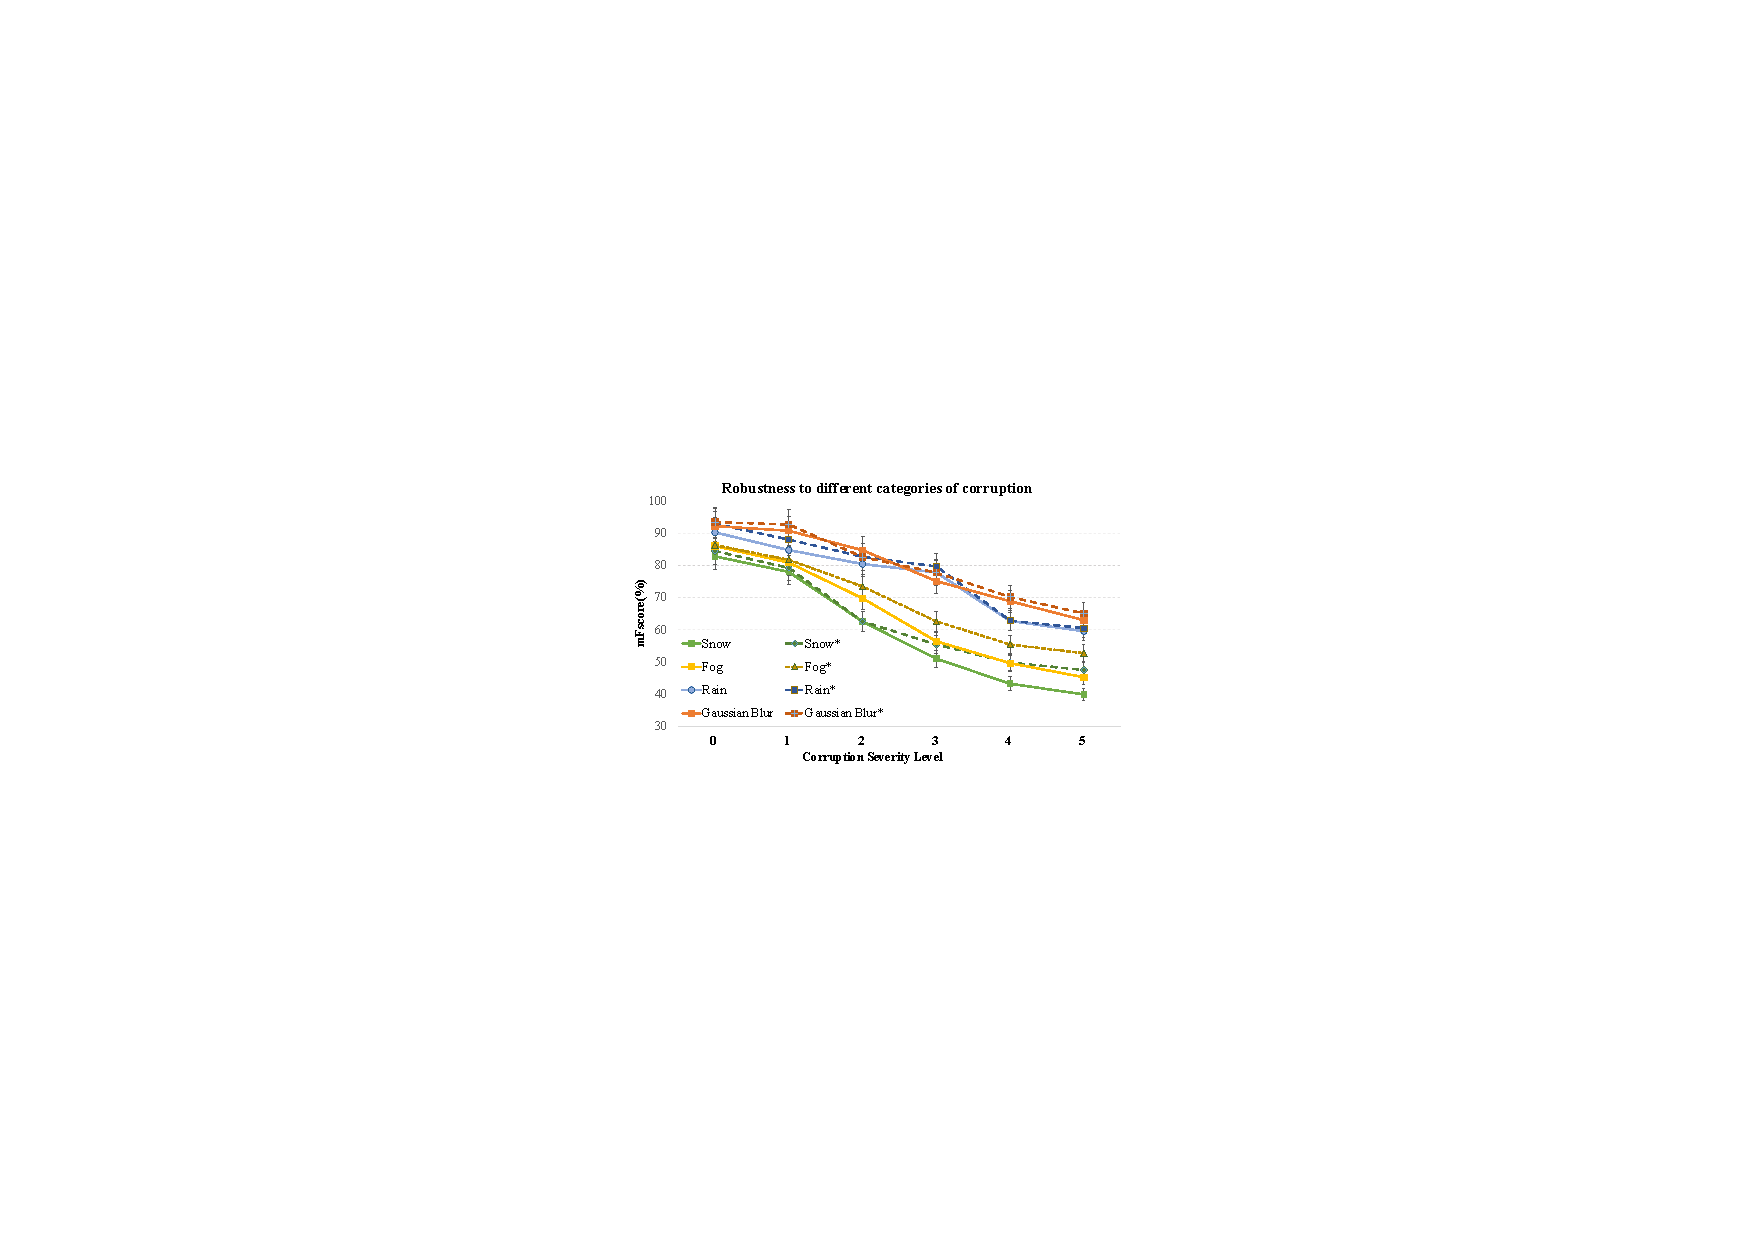
\includegraphics[
        width=\columnwidth]{dataPlot2}
    \caption{Model performance with regard to various corruptions.}
    \label{dataPlot}
\end{figure}
\begin{figure}[!htbp]
    \centering
    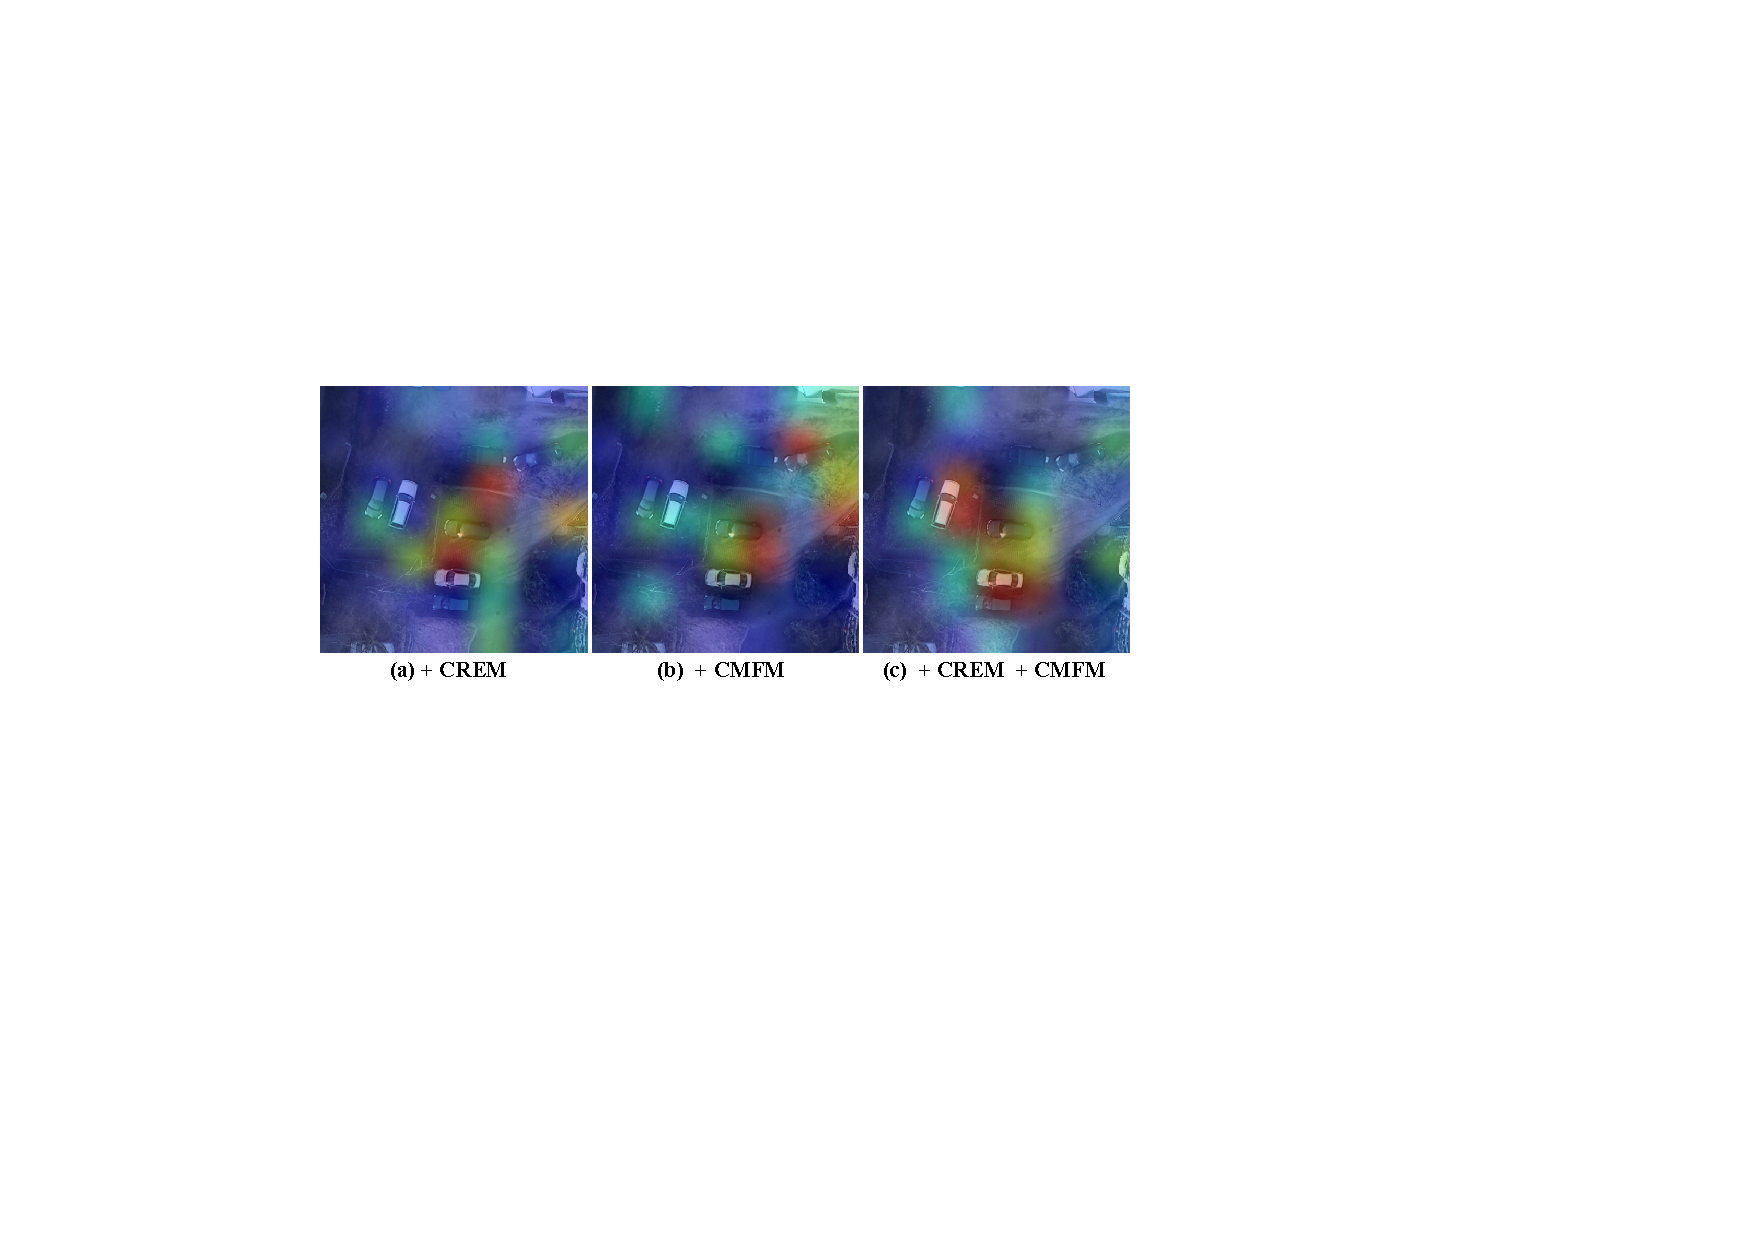
\includegraphics[width=\columnwidth]{attentionMap.pdf}
    \caption{The generated heat map associated with Car. 
    }
    \vspace{-0.38cm}
    \label{attentionMap}
\end{figure}
\begin{figure*}[!htbp]
    \centering
    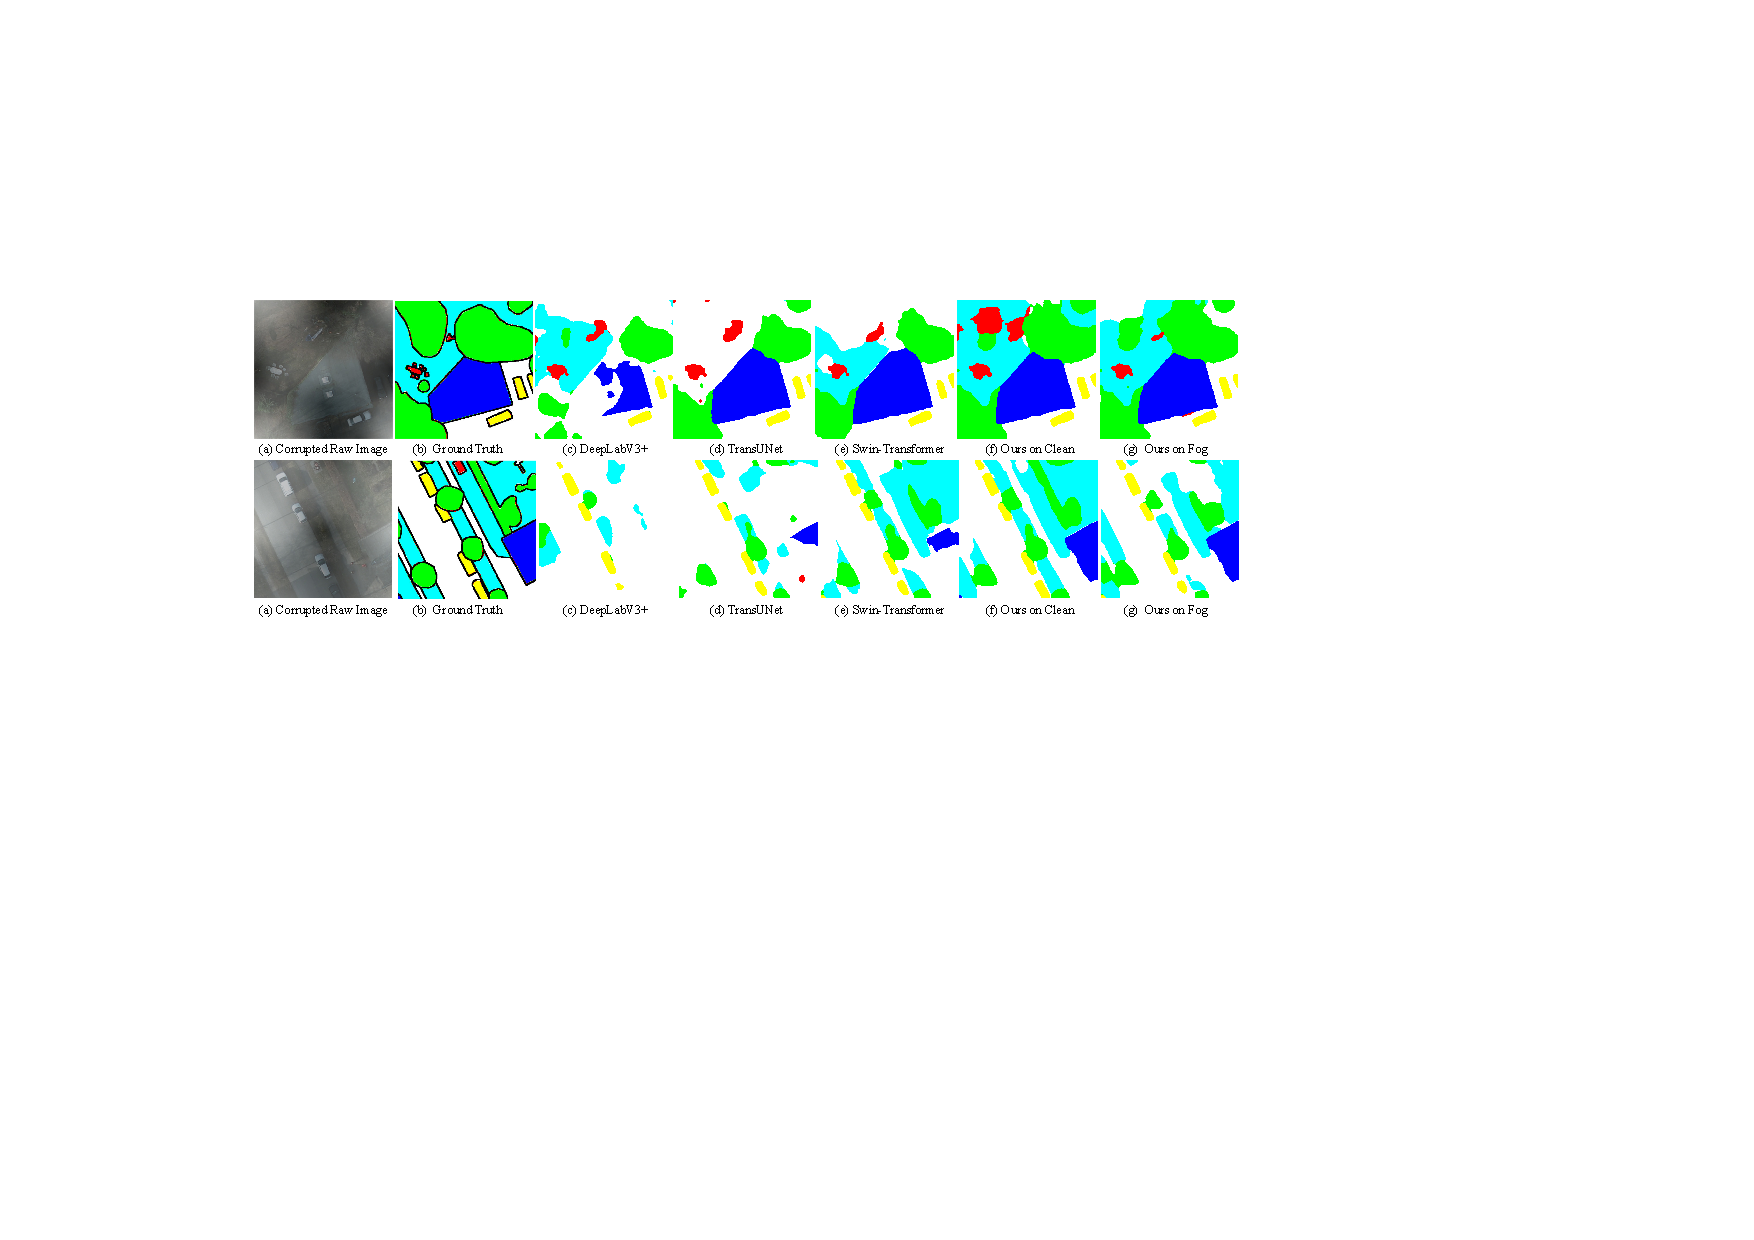
\includegraphics[width=\textwidth]{visualResult.pdf}
    \caption{Qualitative comparisons of several approaches for semantic segmentation of RSIs. The original image is corrupted by the fog of severity level three.
    }
    \label{visualResult}
\end{figure*}
This section is to compare the effect of proposed constituent. We integrate each part into the backbone with \emph{A} as the reference. According to \emph{A} and \emph{B} in Table.\ref{cremAbla}, when performing downstream semantic segmentation tasks, ConvNeXt achieves 3.42\% better classification accuracy and 2.78\% better robustness than Segformer\cite{xieSegFormerSimpleEfficient2021} as SOTA. The cross comparison between \emph{A} with \emph{C, D,} and \emph{E} reveals that SCLA contributes most in terms of improving classification accuracy and robustness (13.86\% reduction in CD). In summary, the model that incorporates all components demonstrates the superior performance (a decrease in CD of 17.49\% and a 3.19\% improvement in mFscore compared to the reference). Table.\ref{cmfmAbla} compares each part of CMFM.  \emph{+SNL} means the Simplifed Nonlocal block, which is derived from GCNet\cite{caoGCNetNonlocalNetworks2019}. The blue dashed box in  Figure.\ref{backbone} is the Fusion module(\emph{FM}).  \emph{Concat} simply concatenates multimodal inputs. It can be concluded from the combination of \emph{A } and \emph{B} in Table.\ref{cmfmAbla} that SNL effectively improves the accuracy and robustness in both clean and foggy conditions. Based on the comparison of \emph{BC} and \emph{BD}, FM improves the classification accuracy and robustness by 4.07\% and 8.17\% respectively in the corrupted environment. The additional query embedding( \emph{+QE}) of dsm makes \emph{E} different from \emph{F}. Despite the 0.2\% improvement under clean, there is an extra 0.83 GLOPs and no reduction in CD. CMFM achieves a balance between efficiency, accuracy, and robustness. 

 Figure.\ref{dataPlot} illustrates the performance with regard to various corruptions in RSIs. \bm{$*$} denotes utilizing the corrupted as well as clean data in the training stage. It is beneficial to enhance robustness while exposing model to both scenes during the training stage. Additionally, our model performs better when coping with Gaussian blur, whereas the performance degrades the most in snow conditions. We also generate the feature map with regard to the class Car in Figure.\ref{attentionMap}. Surrounding pixels can be well activated. With the aid of the effective multimodal fusion, our model is characterized with strong robustness due to the improved generalization of capturing long-range dependencies. 

\subsubsection{Comparison Study}
Table.\ref{compTable} shows result of the comparison study. Our model performs best for Car among all classes. TRM, which is the second best, is outperformed by 6.7\% in mFscore under fog and 2.26\% in CD value. We also observe that Transformer-based methods tend to perform better under clean, while the performance degradation is more severe in foggy conditions. This is attributed to the fact that CNN methods possess better induction bias, while ViTs require more data as pre-training to improve generalization. Our model has better performance in terms of accuracy and robustness compared with other SOTAs.

\section{CONCLUSION}
In this letter, we design a robust network for LCC in foggy conditions. Based on ConveNext, we propose CREM and CMFM based on attention mechanism and multimodal fusion to enhance robustness. The ablation study and comparison experiment demonstrate that our model is robust to fog corrupted RSIs, maintaining a balance between accuracy and robustness. It is our hope that this inspiring letter will provide an opportunity for researchers to explore the robustness in the field of remote sensing and earth observation more generally.

%  \newpage
\bibliography{IGRLRef}
\bibliographystyle{IEEEtran.bst}

\end{document}


